\documentclass[report.tex]{subfiles}
\begin{document}
This chapter describes the experimental setup that aims to validate the
implementation and test the hypotheses introduced in Section \ref{sec:hypotheses}.
Firstly, the assumptions and parameters that are the basis of the simulations are described.
Second, datasets and methods that are used to test the hypotheses are
elaborated.

\section{Neuron parameters}
Since the neural network topologies between the backends are shown to be similar,
the parameters related to this topology are shared as well.
By applying the theory from \textcite{Rueckauer2017} (see section
\ref{sec:coding}), this section will explain how input data, network weights,
and network biases can be transferred from \glspl{ANN} to \glspl{SNN}.
It will then proceed to describe the setup with which prepares the scene for the
experimental results in the following chapter.

As explained in Section \ref{sec:coding}, normalised input in \glspl{ANN} can
be inserted into \glspl{SNN} with the help of a linear transformation.
This transformation has been examined empirically, by constructing a simple 
one-neuron network, and injecting a constant current over time.
By running a number of experiments, it is possible to measure the integrated
current in the neuron and the amount of spikes it produces over time.

\begin{figure}
  \centering
  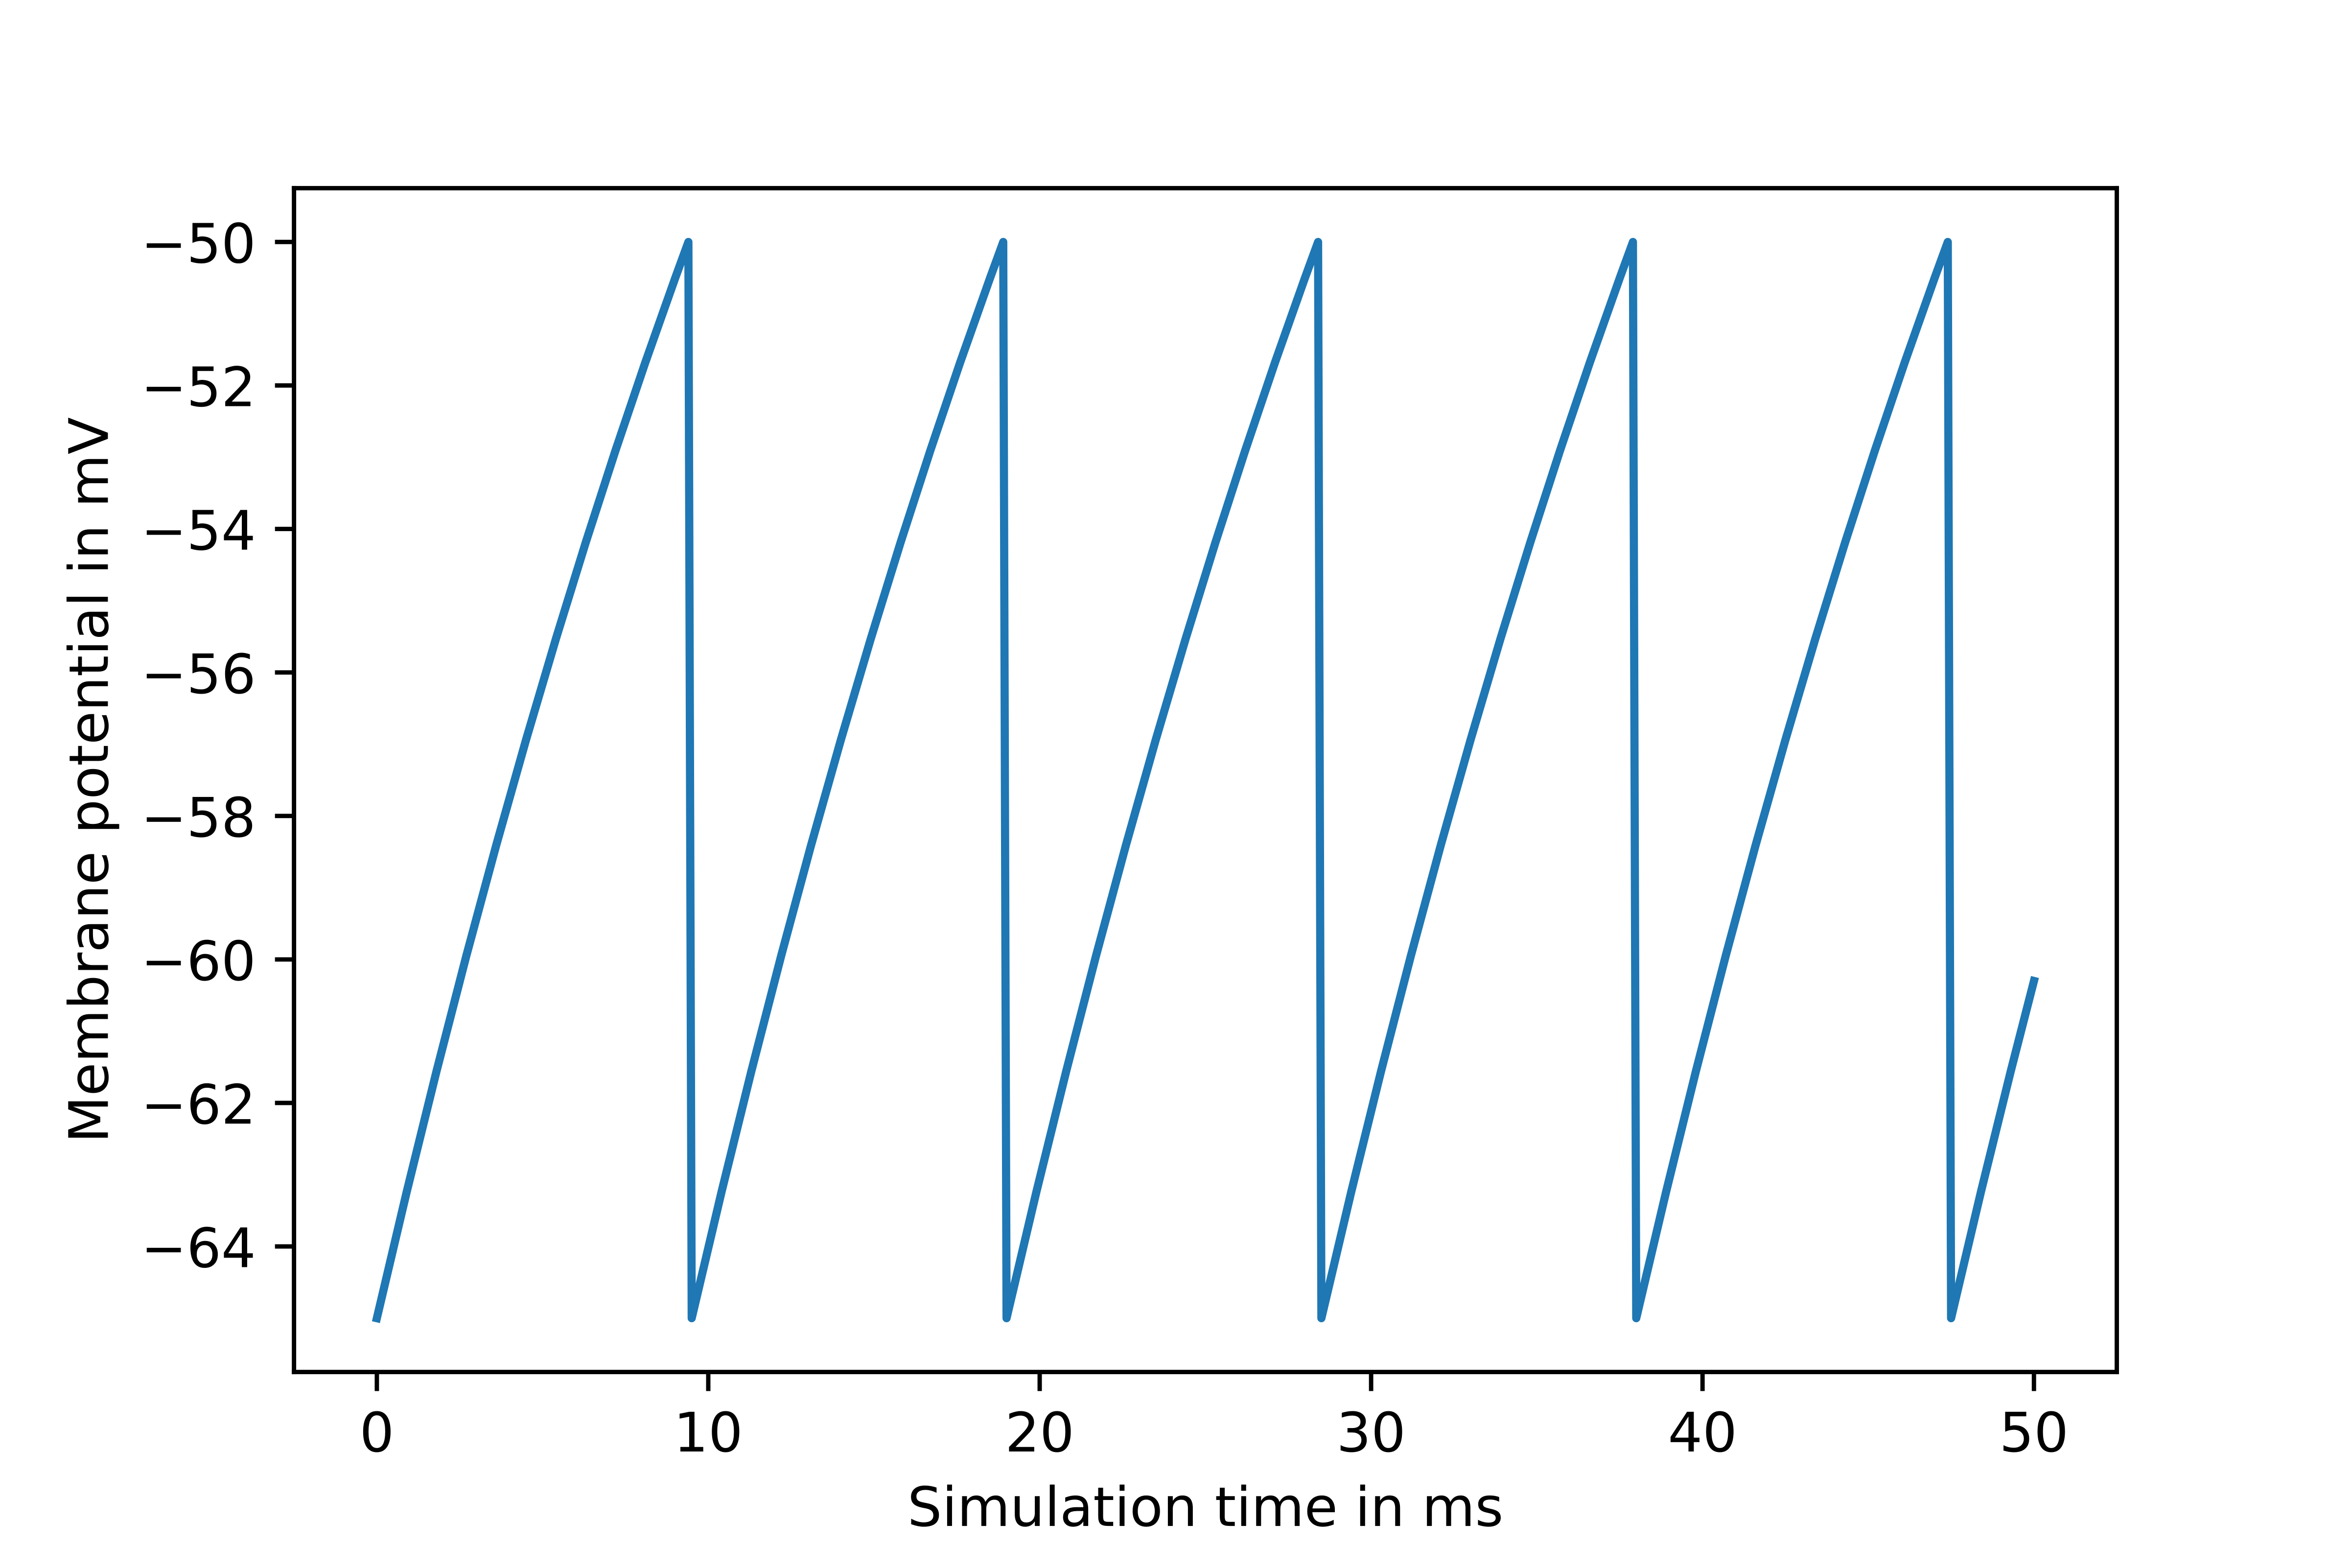
\includegraphics[width=0.8\textwidth]{images/membrane.png}
  \caption{Membrane potential for a LIF neuron given a constant input current of
  2 nA, simulated over 100 ms.}
  \label{fig:membrane}
\end{figure}

Figure \ref{fig:membrane} shows one such experiment, in which the membrane
potential of a single neuron is plotted over time.
The neuron is given a constant input current of 1.3 nA, and 
produces 5 spikes during the 100 ms simulation time. 
As expected in section \ref{sec:coding}, the interspike interval is constant.

A neuron only spikes when its membrane potential exceeds its excitation threshold
$V_{thr}$, but depends on a number of parameters to describe the neuron
conductivity, current decay time etc.
In ll three, PyNN, NEST and BrainScaleS, these parameters can be programatically
defined. Table \ref{tab:neuron_parameters} shows the default parameters for
NEST (also shown in Listing \ref{lst:lif-cond-exp}).
The $\tau_{syn}$ parameters denote the decay time for the input spike currents. 
Similarly, the membrane time constant, $\tau_m$, expresses the time it takes for the
neuron membrane to decay to its resting state ($V_{rest}$) if no other
input arrives. 
For the LIF\index{neuron model!leaky-integrate-and-fire} model used in PyNN,
all $\tau$ parameters decay exponentially \cite{Davison2009}.
The $V_{rev}$ parameters explain the potential to integrate into the neuron,
when either excitatory or inhibitory input arrives. 

\renewcommand{\arraystretch}{1.3} 
\begin{table}
\begin{tabular}[center]{l r l l}
  \hline
  $C_m$ & 1 & nF & Capacity of the membrane. \\ \hline
  $I_{offset}$ & 0 & nA & Offset current. \\ \hline
  $V_{rest}$ & -65 & mV & Resting membrane potential. \\ \hline
  $V_{reset}$ & -65 & mV & Reset potential after a spike. \\ \hline
  $V_{rev}^E$ & 0 & mV & Reverse potential for excitatory input. \\ \hline
  $V_{rev}^I$ & -70 & mV & Reverse potential for inhibitory input. \\ \hline
  $V_{thr}$ & -50 & mV & Spike threshold. \\ \hline
  $\tau_m$ & 20 & ms & Membrane time constant. \\ \hline
  $\tau_{refrac}$ & 0.1 & ms & Duration of the refractory period. \\ \hline
  $\tau_{syn}^E$ & 5 & ms & Decay time of the excitatory synaptic conductance. \\ \hline
  $\tau_{syn}^I$ & 5 & ms & Decay time of the inhibitory synaptic conductance. \\  \hline
\end{tabular}
\caption{The names, default values and description of the neuron parameters in
PyNN, NEST and BrainScaleS.}
\label{tab:neuron_parameters}
\end{table}

With the exception of $I_{offset}$, which is the constant input current,
the parameters are kept constant in Volr, and used in all spiking backends
to avoid spurious influences.


\section{Parameter translation} \label{sec:translation}

As described in Section \ref{sec:coding} it is necessary to discover the exact
linear relationship between \gls{ANN} activations and \gls{SNN} activations, and
this section provides the empirical basis for the input and weight normalisation
rates that are used in the remainder of the thesis.

The code for the experiments and visualisations are available in Appendix
\ref{app:verification}.

Figure \ref{fig:spike_rates} plots the spike count and spike rate against the
constant input current, using the neuron parameters from Table \ref{tab:neuron_parameters}.
120 simulations have been performed with offset currents ranging from 0 to 12, 
using a resolution of 0.1.

\begin{figure}
  \centering
  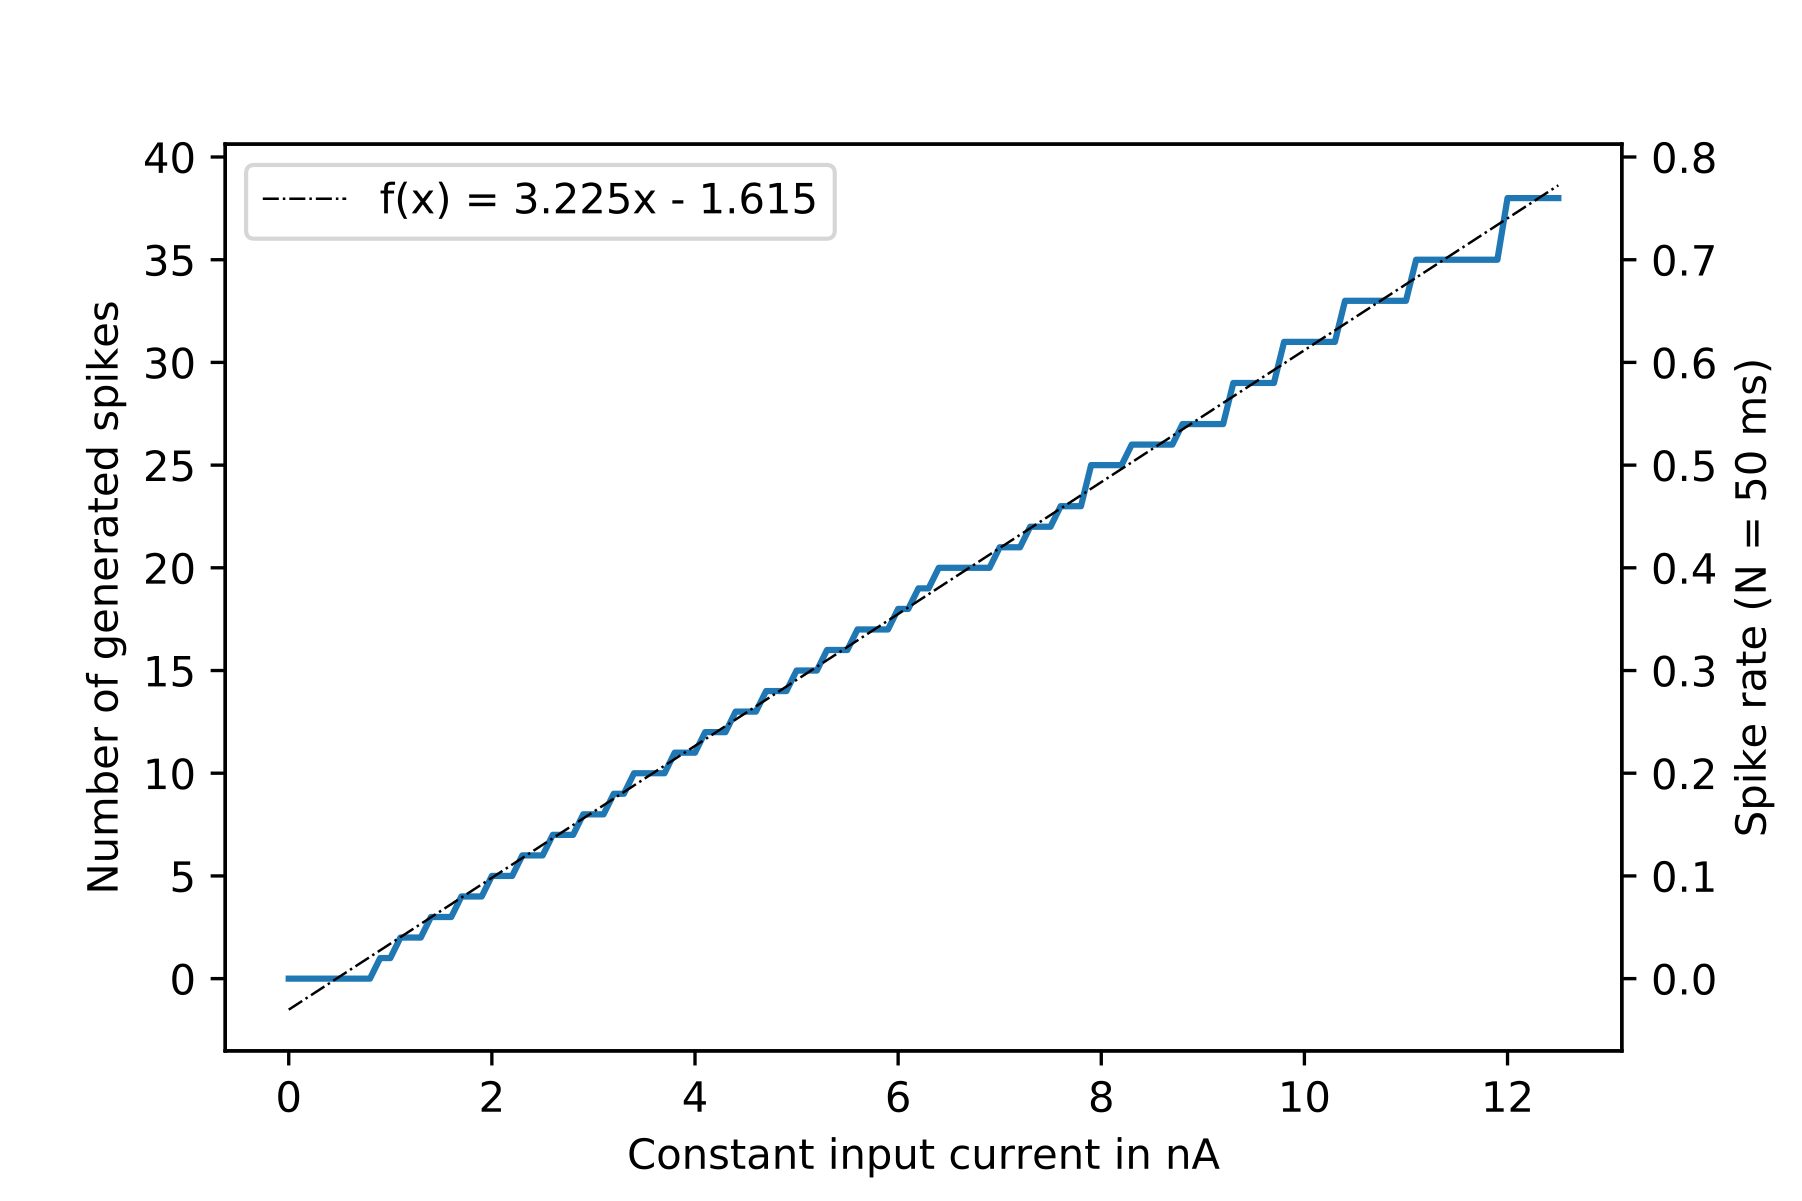
\includegraphics[width=0.7\textwidth]{images/spike_rate.png}
  \caption{Spike count and spike rates of a single neuron from 120 simulations of 50 ms
    duration with varying input current offset ($[0;12]$).
  A linear regression ($r^2$ = 0.9977) shows the best-fit linear model.}
  \label{fig:spike_rates}
\end{figure}

The relationship shows that there is an approximated linear correlation, when the
input current is kept below 12 and above 1. 
Outside this range the relationship becomes unstable: towards 0 it flatlines and
produces no spikes, and towards and beyond 12 it begins to resemble a non-differentiable 
step function.
Cropping the `unstable' parts of the graph away produces spike-counts in the interval
$[1;38]$ and spike rates in the interval $[0.02;0.76]$.
In order to allow compositions of populations, as required by the \gls{DSL},
future populations will have to scale their stimuli to fit the same intervals.
Otherwise the assumption about a linear correlation between input stimuli and
output rates collapses, and the differentiation becomes imprecise.
In turn, this will result in bad prediction rates for the model, because it
cannot properly learn from the backpropagation errors.

To illustrate this point in a deeper network, Figure
\ref{fig:spike_rates_not_weighted} shows
three populations
--each with a single neuron---chained
through synapses to the first population, whose spike rates are seen above.
Each datapoint is a separate simulation over 50ms with a fixed
current offset for the first population.
The first population is synaptically connected to the second population, which 
integrates the spike currents, until that population fires and so on.
Without weight normalisation, the correlation is visibly unstable.
All weights and biases between the populations are set to a constant value of 1
and 0 respectively.

\begin{figure}
  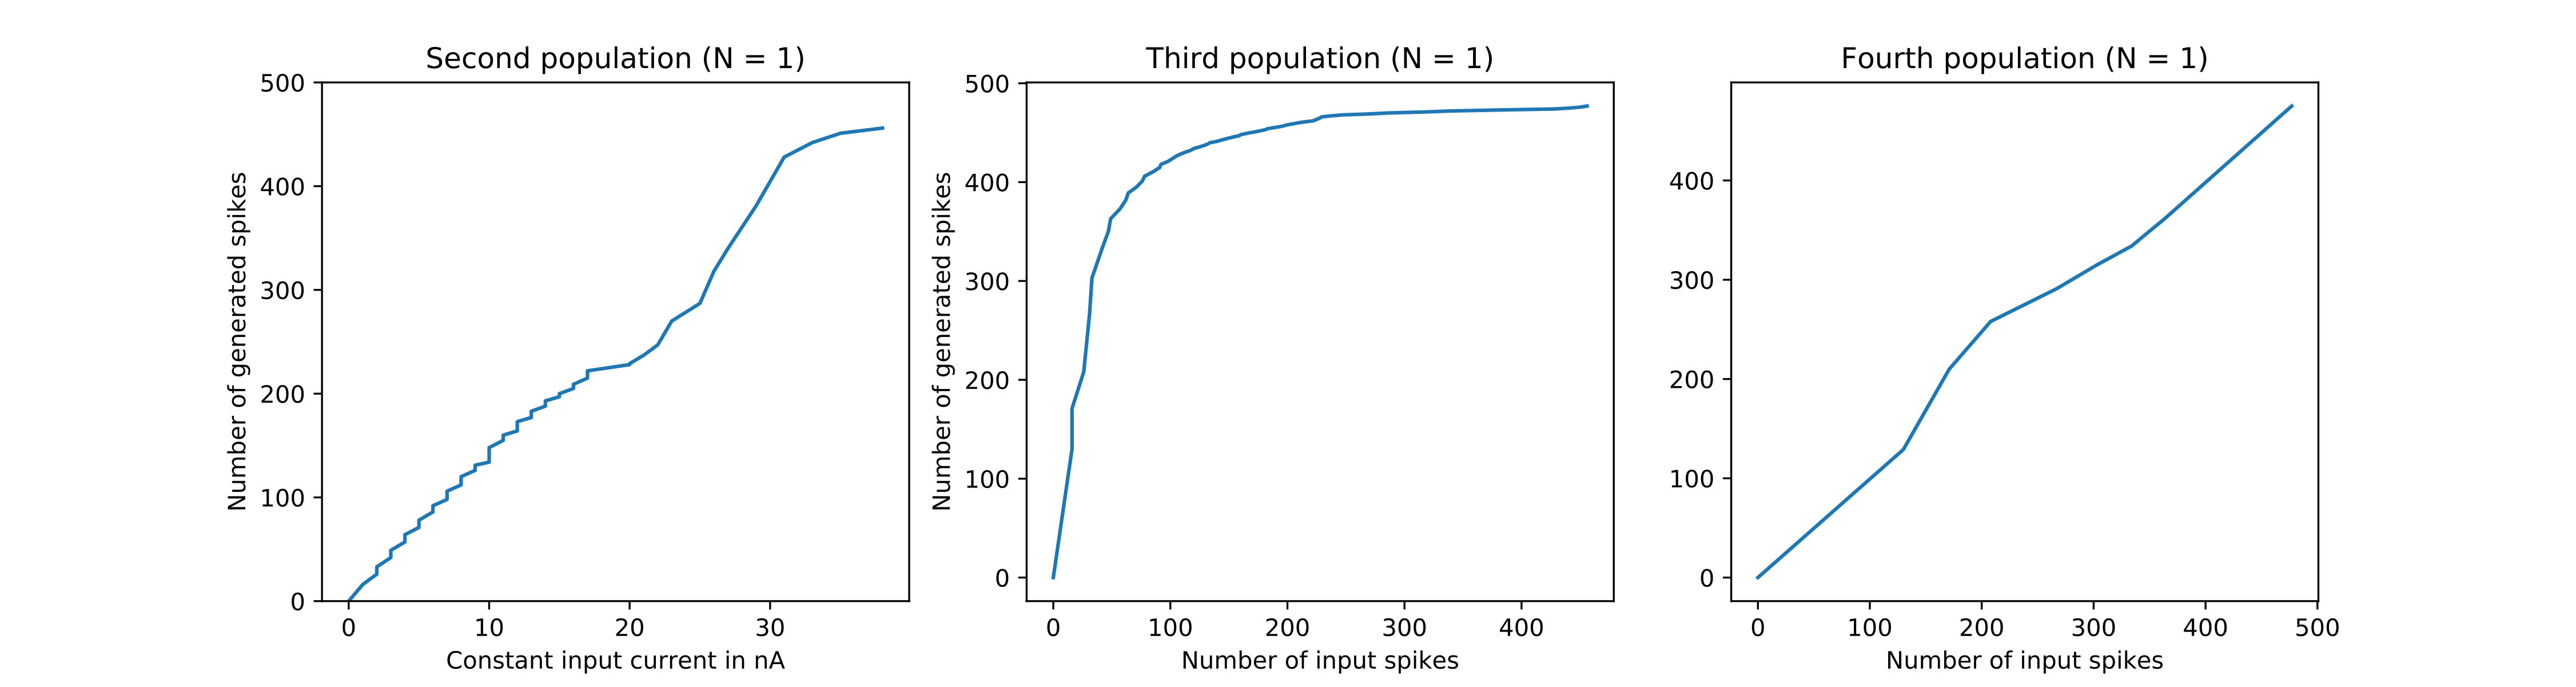
\includegraphics[width=\linewidth]{images/spike_rate_not_weighted.png}
  \caption{Spike counts for a second, third and fourth population in a chained network of
  single-neuron populations with a constant synaptic weight of 1.}
  \label{fig:spike_rates_not_weighted}
\end{figure}

The correlations are clearly not linear.
To avoid this it is possible to adjust the weights between the population
through an approximation of
the weight normalisation scheme from \textcite{Rueckauer2017}, shown in Equation
\ref{eq:weight_norm}.
The normalisation is based on the maximum activation of the previous layer.
Figure \ref{fig:spike_rates} illustrates that this relation is linear.
However, in deeper layers the activation is scaled by the number of previous
neurons, since the post-synaptic potentials accumulates.
In the case of the NEST and BrainScaleS backends,\index{NEST}\index{BrainScales}
the post-synaptic potentials are solely depending on the synaptic weights
\cite{Gewaltig2007, Schmitt2017}.
In other words they are not subject to the laws of physics, and
the energy of the spikes does not depend on the amount of post-synaptic
neurons.
For the post-synaptic neurons this means that the input potential for a neuron
is linearly correlated with the number of pre-synaptic connections.

A number of experiments has been conducted to find the appropriate scaling values,
and, given a population of size $N^l$ and its preceding population of size $N^{l-1}$,
a normalisation value of $w_{N^l} = 0.065 / N^{l-1}$
has been shown to provide a stable linear approximation of spike rates in a
network.
Figure \ref{fig:spike_rates_chain} shows the same populations as in 
Figure \ref{fig:spike_rates_not_weighted} with the same constant weights of 1, but with
the normalisation term applied.

\begin{figure}
  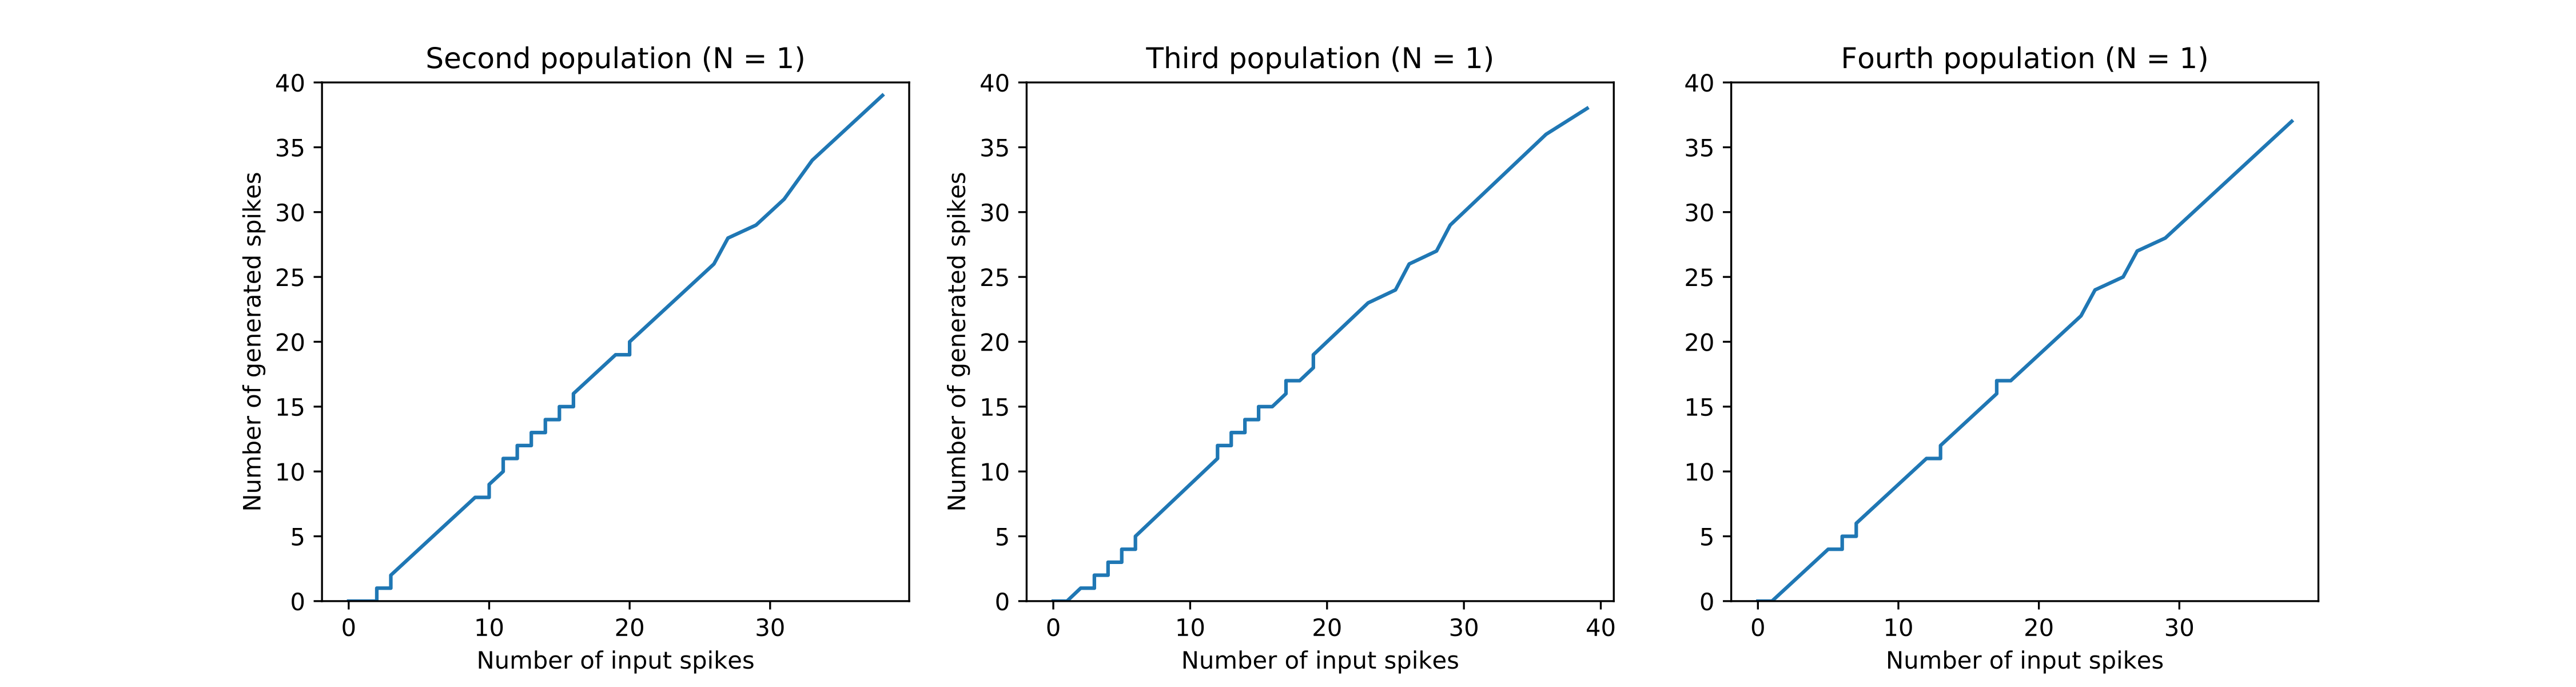
\includegraphics[width=\linewidth]{images/spike_rate_chain.png}
  \caption{Spike counts for the second, third and fourth population in a chained network of
  single-neuron populations, adjusted for previous neuron activation with the
  normalisation term $0.065 / N^{l - 1}$.}
  \label{fig:spike_rates_chain}
\end{figure}

To prove this in larger networks, the same normalisation term was applied to an MNIST
topology of (\texttt{\textbf{dense} 100 100 $\obar$ \textbf{dense} 100 10}).
Figure \ref{fig:spike_rates_mnist} shows the averaged spike rate for each neuron
population, with normalised weights.
The figure shows that a near-linear relationship exists, even for larger neuron populations.

\begin{figure}
  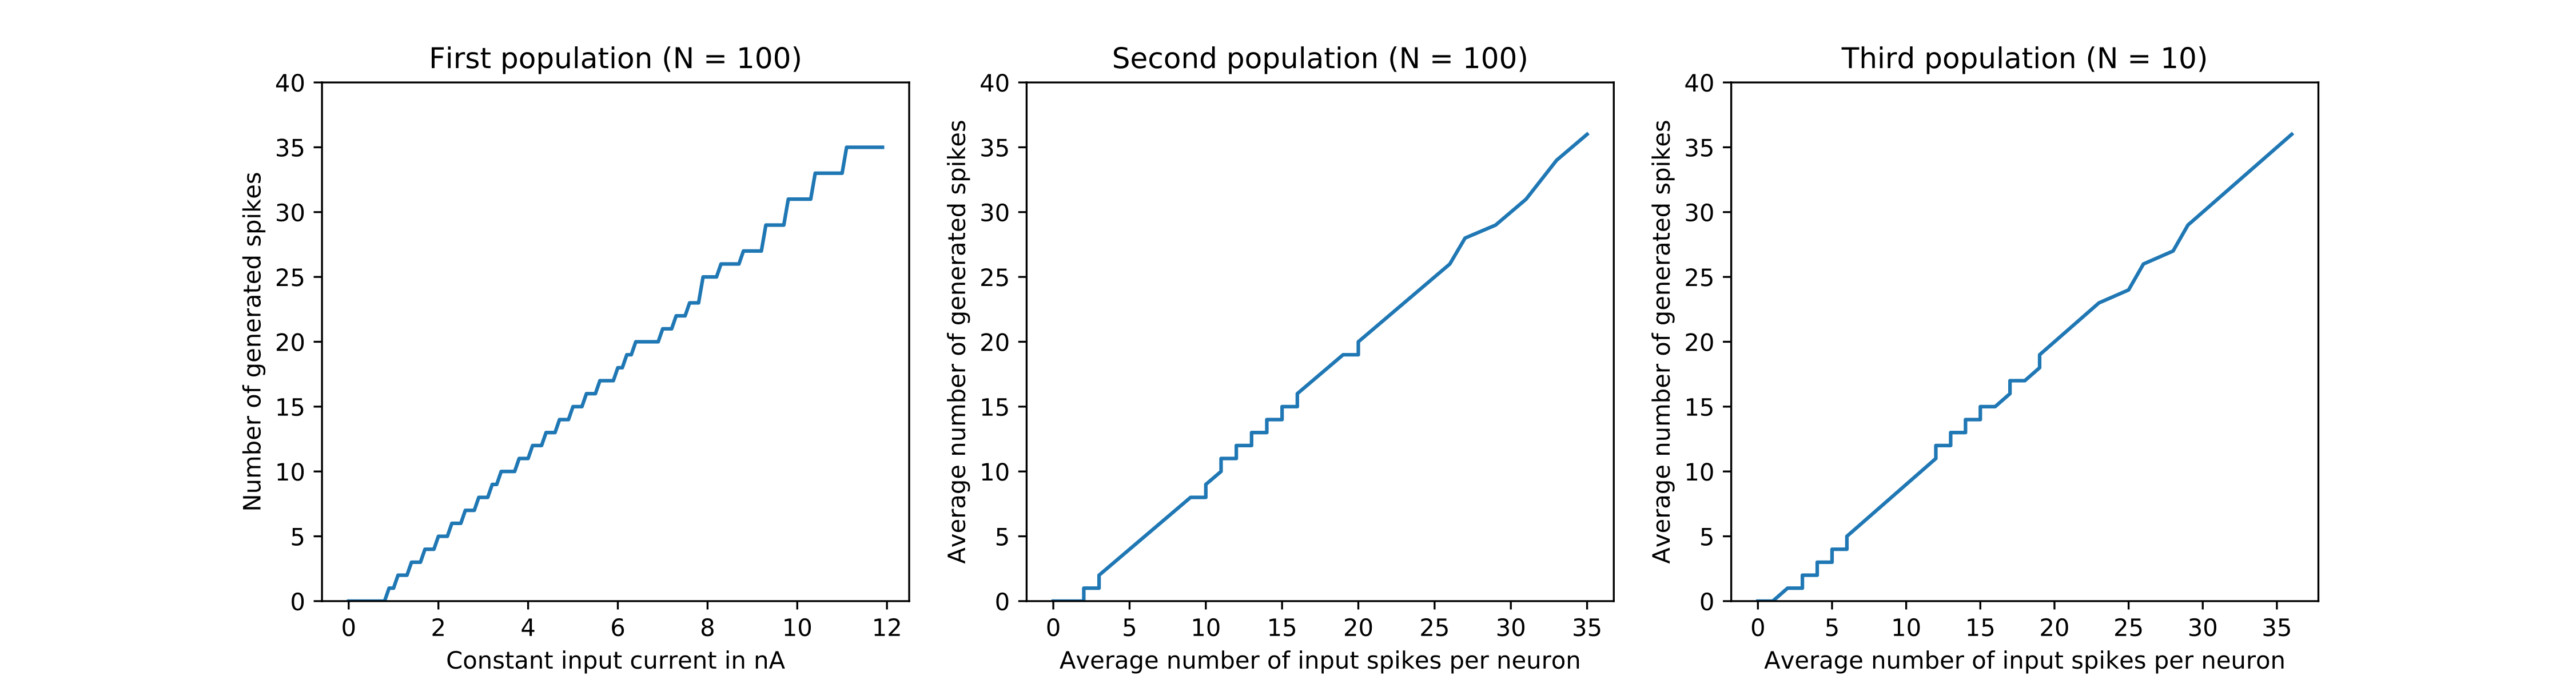
\includegraphics[width=\linewidth]{images/spike_rate_mnist.png}
  \caption{Spike count for the first, second and third population in an MNIST
    network, adjusted for previous neuron activation with the
  normalisation term $0.065 / N^{l - 1}$.}
  \label{fig:spike_rates_mnist}
\end{figure}

For network training in the remainder of the thesis, this normalisation will
be applied after the weights have been calculated through regular backpropagation. 
This separates the weight normalisation from the actual \gls{SNN} weights, such
that the optimisation operates on the idealised linear spike rate model.
Listing \ref{lst:layer_norm} shows the separation of concerns within the densely
connected spiking layer, where the raw weights are stored directly, and the normalised
weights are set for the neuron projection that connects the input and output
populations.

\begin{lstlisting}[language=Python,label={lst:layer_norm},caption={Weight
normalisation in the spiking dense layer.}]
def set_weights(self, weights): 
    self.weights = weights
    normalised = self._normalise_weights(weights)
    self.projection.set(weight=normalised)   
\end{lstlisting}



\section{Problem sets}
Three problem sets will be tested: the NAND ($\neg(A \land B)$) and XOR
($\oplus$) logical gates, as well as the 
Modified National Institute of Standards and Technology
(MNIST) database\index{MNIST}.
The NAND and XOR problems are trivial for \glspl{ANN} to learn, and are used as
a means to test and compare the rudimentary learning capacities of the NEST
backend.

The NAND and XOR experiments will be based on the same network topology
(\texttt{\textbf{dense} 2 4 $\obar$ \textbf{dense} 4 2}). 
All backends will execute the experiment with randomly initialised weights. However, the spiking backends will be evaluated
a second time with imported weights and biases from the optimised Futhark
networks.
This is interesting because Futhark is expected to outperform the \glspl{SNN}, and since the
network topology is shared, network parameters can be inserted 1:1.
In theory this should improve the initial training of the spiking models and
lead to an increased accuracy.

The weights and biases from the optimised Futhark model will only be imported into NEST,
which then trains the weights to fit the spiking neuron model.

The MNIST dataset is widely used for training neural networks to classify
images of digits between 0 and 9. 
It is also commonly used for implementation benchmarks \cite{Schmidhuber2014,
Schmitt2017}, with the best networks scoring an error rate of 0.21\%
\cite{LeCun2019}.
MNIST consists of a collection of 60,000 training images and 10,000 testing images of handwritten digits \cite{LeCun1998}.

To predict the MNIST digits two networks will be constructed.
MNIST images contain 784 pixes (28x28), but to avoid too complex simulations
it is necessary to limit the network size.
The images have been cropped and scaled to 10x10 pixels, such that the initial
network layer can be scaled to 100 neurons.
The topology for the sequential model is 
\texttt{\textbf{dense} 100 100 $\obar$ \textbf{dense} 100 10}.

To test the parallel structures of the \gls{DSL}, a second and parallel network
will be constructed.
The network will resemble the sequential model, but consist of two separate
parallel subnetworks (\texttt{\textbf{dense} 20 10}), that is merged to produce
an output of 20 neurons.
The full model is as follows:
\texttt{\textbf{dense} 100 20 $\obar$ (\textbf{dense} 20 10 $\ominus$\
\textbf{dense} 20 10) $\obar$ \textbf{dense} 20 10}.
The idea of the model is that the two parallel subsystems can learn semantically
different tasks, and the final layer will be able to `choose' which subnetwork to
use, based on its weights.

\section{Experiment method}
All the above mentioned experiments are classification tasks, and the labels
are encoded as one-hot vectors.
To compare the network output with the labels, the argmax value of the network
output is taken and converted to a one-hot vector of the same shape as the label
data.

To avoid one-off effects such as local minima or (un)fortunate weight
initialisation, all experiments have been repeated 10 times.
The results reported below are accumulations of the prediction accuracies
and errors from the runs.

Weights have been initialised in the models using a normal distribution with a
mean of 1 and a standard deviation of 1.

The experiments use a 80/20 training/testing split with a fixed learning rate of
0.1, and the batch size has been set to 64.

To make the experiments as reproducible as possible, they have all been
initialised with constant random seeds.
Since all randomness in Futhark is based on this seed, all results are constant and
standard deviations are effectively 0.
This is not the case in PyNN, where the randomness is highly backend-specific.
A configuration for setting the initial seed exists
(\texttt{rng\_seed\_seeds})---and have been set for all experiments---but
PyNN does not fully support the randomness configurations in NEST
\cite{Gewaltig2007}.

\end{document}
